\chapter{Conditions and Signals} 

In the previous chapter, we saw how we could use a lock to provide mutual
exclusion.  This technique allows us to implement many concurrent objects,
including total concurrent datatypes.  However, it is not enough to implement
a partial concurrent datatype, where a thread might have to wait until some
condition becomes true, or a synchronisation object, where a thread might have
to wait for another thread with which to synchronise. 

For example, consider a partial queue.  Here, if a thread attempts to dequeue
when the queue is empty, it should wait until the queue becomes nonempty.
During this time, we would like the thread to \emph{suspend}, and so stop
using computational resources.  When another thread does enqueue a value, it
should signal to the suspended thread, so that it can resume.  

In order to achieve this, we need a wait/signal mechanism.  In SCL, this is
provided by \emph{conditions}.  If |lock| is a |Lock|, then
\begin{scala}
  lock.newCondition
\end{scala}
creates a new |Condition| object associated with |lock|.  
Each condition has operations as follows:
%
\begin{itemize}
\item |await()|: suspend, giving up the lock, wait for a signal on the
  condition, and then re-acquire the lock;

\item |signal()|: signal to a thread waiting on this condition;

\item |signalAll()|: signal to all threads waiting on this condition.
\end{itemize}
%
Each operation should be performed while holding the related |Lock|. 

Figure~\ref{fig:MonitorPartialQueue} uses this technique to implement a
partial queue.  (The helper trait |PartialQueue1| gives a default no-op
implementation of the |shutdown| operation.)  Here, a |Lock| is used for
mutual exclusion.  In addition, a |Condition| |notEmpty| is used to allow a
|dequeue| that cannot proceed, because the queue is empty, to wait, which
releases the lock.  A thread that performs an |enqueue| then signal on
|notEmpty| to indicate that the queue is now not empty.  The waiting thread
that receives the signal then has to wait to reacquire the lock, which is done
as part of the |await| operation.  It then needs to re-check whether the queue
is empty: it is possible that another thread performed a |dequeue|, after this
thread received the signal but before it acquired the lock, and so re-emptied
the queue.

%%%%%

\begin{figure}
\begin{scala}
trait PartialQueue1[T] extends PartialQueue[T]{
  def shutdown() = {}
}

class MonitorPartialQueue[T] extends PartialQueue1[T]{
  /** The queue itself. */
  private val queue = new Queue[T]

  /** A monitor object, to control the synchronisations. */
  private val lock = new Lock

  /** Condition for signalling that the queue is not empty. */
  private val notEmpty = lock.newCondition

  /** Enqueue £x£. */
  def enqueue(x: T) = lock.mutex{
    queue.enqueue(x)
    notEmpty.signal() // Signal to a waiting dequeue.
  } 

  /** Dequeue a value.  Blocks until the queue is non£-£empty. */
  def dequeue(): T = lock.mutex{
    while(queue.isEmpty) notEmpty.await() // Wait for a signal.
    queue.dequeue()
  }
}
\end{scala}
\caption{A partial queue implemented using a {\scalastyle Condition}.}
\label{fig:MonitorPartialQueue}
\end{figure}

%%%%%

\begin{instruction}
Study the details of the implementation. 
\end{instruction}

The term \emph{monitor} is often used to describe a concurrent object,
encapsulating data and operations on that data, providing mutually exclusive
access to the data, together with a wait/signal mechanism.  We will see
another implementation of monitors, provided by the Java Virtual Machine, in
Chapter~\ref{chap:JVMMonitors}, and a further implementation, using
semaphores, in Chapter~\ref{chap:semaphores}.   

It is very common for a thread to have to wait until some property becomes
true.  SCL |Conditions| include an operation |await(test)| that waits until
|test| becomes true.  It is defined as follows (remember that the type
signature means that |test| is passed by name, so evaluated only in the body
of the operation, on each iteration of the loop):
%
\begin{scala}
  def await(test: => Boolean): Unit = while(!test) await()
\end{scala}
%
Thus the |dequeue| operation could be written more succinctly as:
\begin{scala}
  def dequeue(): T = lock.mutex{
    notEmpty.await(queue.nonEmpty) // Wait for a signal.
    queue.dequeue()
  }
\end{scala}

Try to choose good names for |Condition|s.  I use the convention that the name
of a |Condition| corresponds to the property that a signal on the condition
indicates, or, equivalently, the property for which a thread waits.  Above, a
signal on |notEmpty| indicates that the queue is not empty; and a |dequeue|
waits on |notEmpty| until the queue is not empty.


%%%%%%%%%%%%%%%%%%%%%%%%%%%%%%%%%%%%%%%%%%%%%%%%%%%%%%%%%%%%

The above partial queue implementation uses a single |Condition|.  However, a
monitor may use multiple |Condition|s.

%%%%%

\begin{figure}
\begin{scala}
class BoundedMonitorPartialQueue[T](bound: Int) extends PartialQueue1[T]{
  /** The queue itself. */
  private val queue = new Queue[T]

  /** A monitor object, to control the synchronisations. */
  private val lock = new Lock

  /** Condition for signalling that the queue is not full. */
  private val notFull = lock.newCondition

  /** Condition for signalling that the queue is not empty. */
  private val notEmpty = lock.newCondition

  /** Enqueue £x£.  Blocks while the queue is full. */
  def enqueue(x: T) = lock.mutex{
    notFull.await(queue.length < bound) // Wait for a space (1).
    queue.enqueue(x)
    notEmpty.signal() // Signal to a waiting dequeue at (2).
  }

  /** Dequeue a value.  Blocks until the queue is non-empty. */
  def dequeue(): T = lock.mutex{
    notEmpty.await(queue.nonEmpty) // Wait for a signal (2).
    val result = queue.dequeue()
    notFull.signal() // Signal to a waiting enqueue at (1).
    result
  }
}
\end{scala}
\caption{A bounded partial queue implemented using {\scalastyle Condition}s.}
\label{fig:BoundedMonitorPartialQueue}
\end{figure}

%%%%%

Figure~\ref{fig:BoundedMonitorPartialQueue} gives an implementation of a
\emph{bounded} partial queue, that can hold at most |bound| values.  Thus an
|enqueue| might have to wait for there to be a space for its value.  This is
implemented using a second |Condition|, |notFull|.  A |dequeue| signals on
this condition when it removes a value, to signal that the queue is not full. 

\begin{instruction}
Study the details of the implementation.
\end{instruction}

We could have written the |dequeue| operation as
%
\begin{scala}
  def dequeue(): T = lock.mutex{
    notEmpty.await(queue.nonEmpty); notFull.signal(); queue.dequeue()
  }
\end{scala}
%
The thread continues to hold the lock after signalling, so it is fine to
signal before dequeueing.  However, the order in
Figure~\ref{fig:BoundedMonitorPartialQueue} seems more logical.

When there are multiple signals in a monitor, it is helpful to make clear
where a particular signal will be received.  In
Figure~\ref{fig:BoundedMonitorPartialQueue}, I have labelled the two |await|s
and |signal|s~``(1)'' and~``(2)'', to help the reader tie them together. 
 % introduction, partial queues (unbounded, bounded)
\section{Implementing a Synchronous Channel}

Conditions can also be used to implement synchronisation objects.  A thread
that needs to synchronise can wait for another thread; when another thread
arrives, it can signal to the waiting thread.  We illustrate the technique by
implementing a basic synchronous channel, to extend the trait in
Figure~\ref{fig:SyncChanT}, with |send| and |receive| operations
that synchronise together.  The channel can be used by an arbitrary number of
senders and receivers.

%%%%%

\begin{figure}
\begin{scala}
trait SyncChanT[A]{
  /** Send £x£, synchronously. */
  def send(x: A): Unit

  /** Receive a value. */
  def receive(): A
}
\end{scala}
\caption{The trait for a synchronous channel.}
\label{fig:SyncChanT}
\end{figure}

%%%%%

The implementation is in Figure~\ref{fig:SharedSyncChan}.  The variable
|value| holds the value currently being sent, or maybe the previous value
sent.  The variable |full| indicates whether the value in |value| is valid,
i.e.~if a current sender is trying to send it. 

%%%%% Check positioning of figure.

\begin{figure}
\begin{center}
\def\height{5.7}
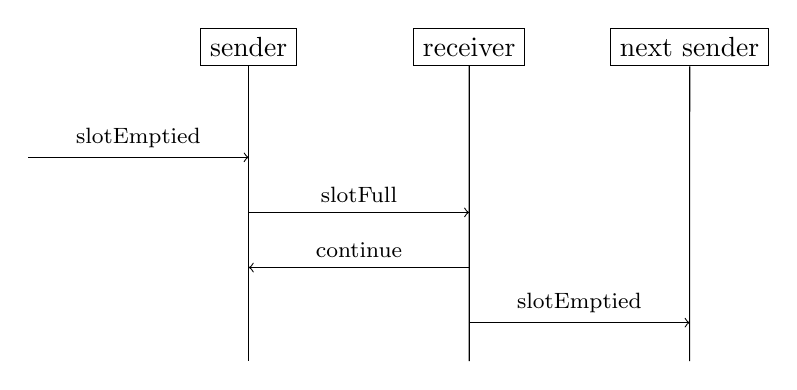
\begin{tikzpicture}[xscale = 2.8, yscale = 0.7]
\draw (0,0) node[draw] (sender) {sender};
\draw (sender) -- ++ (0,-\height);
\draw (1,0) node[draw] (receiver) {receiver}; 
\draw (receiver) -- ++ (0,-\height);
\draw (2,0) node[draw] (sender2) {next sender};
\draw (sender2) -- ++ (0,-\height);
%
\draw[<-] (sender) ++ (0,-2) -- 
  node[above]{\scalashape\footnotesize slotEmptied} ++ (-1,0); 
\draw[->] (sender) ++ (0,-3) -- 
  node[above]{\scalashape\footnotesize slotFull} ++ (1,0);
\draw[->] (receiver) ++ (0,-4) --
  node[above]{\scalashape\footnotesize continue} ++ (-1,0);
\draw[->] (receiver) ++ (0,-5) --
  node[above]{\scalashape\footnotesize slotEmptied} ++ (1,0);
\end{tikzpicture}
\end{center}
\caption{A sequence diagram illustrating the signals in the implementation of
  a synchronous channel.}
\label{fig:syncChan-seqDiagram}
\end{figure}

%%%%%

\begin{figure}
\begin{scala}
class SharedSyncChan[A] extends SyncChanT[A]{
  /** The current or previous value. */
  private var value = null.asInstanceOf[A]

  /** Is the current value of £value£ valid, i.e. ready to be received? */
  private var full = false

  /** Monitor for controlling synchronisations. */
  private val lock = new Lock

  /** Condition for signalling to sender that a value has been deposited. */
  private val slotFull = lock.newCondition

  /** Condition for signalling to current receiver that it can continue. */
  private val continue = lock.newCondition

  /** Condition for signalling to the next sender that the previous value has
    * been read. */
  private val slotEmptied = lock.newCondition

  def send(x: A) = lock.mutex{
    slotEmptied.await(!full) // Wait for previous value to be consumed (1).
    value = x; full = true   // Deposit my value.
    slotFull.signal()        // Signal to receiver at (2).
    continue.await()         // Wait for receiver (3).
  }

  def receive(): A = lock.mutex{
    slotFull.await(full)               // Wait for sender (2).
    continue.signal()                  // Notify current sender at (3).
    full = false                       // Clear the slot.
    slotEmptied.signal() // Clear value, and notify next sender at (1).
    value
  }
}
\end{scala}
\caption{The implementation of a synchronous channel.}
\label{fig:SharedSyncChan}
\end{figure}

%%%%%

We require three conditions for signals between threads:
%
\begin{itemize}
\item Each sender will signal to a receiver on |slotFull| that it has
  deposited a value, which the receiver can take;

\item The receiver will then signal back to the sender on |continue| that it
  can continue; this makes the channel synchronous;

\item The receiver will signal to a sender for the next round on |slotEmptied|
  that it has cleared the value, so that sender can deposit its value.
\end{itemize}
%
Figure~\ref{fig:syncChan-seqDiagram} illustrates the sequence of signals.

The sender waits, on |slotEmptied|, until the previous exchange is complete.
Note that it needs to recheck |full| when it receives a signal on, in case
another sender has run in the meantime and filled the slot.  It then deposits
its value, and signals to a waiting receiver on |slotFull|.  Finally, it waits
for a signal back on |continue|.  Note that there is no need to recheck |full|
at this point, as it cannot be preempted by another sender. 

The receiver waits, on |slotFull|, for a value to be deposited.  It again
needs to recheck |full| when it receives a signal, in case another receiver
has run in the meantime and taken the value.  It then signals back to the
sender on |continue|, clears the slot, and then signals to the next sender on
|slotEmptied|. 

\begin{instruction}
Study the details of the implementation.  Make sure you understand why each of
the signals is necessary.
\end{instruction}


We can test this implementation by running some threads that perform sends and
receives, and log the call and return of each operation.  For simplicity, we
arrange that every send is of a different value.  This makes it easy to
identify matching sends and receives (if they exist).  We then check that the
two invocations overlap.  

As in Section~\ref{sec:exchanger}, it is sound to assume the values sent are
all different, because the implementation is \emph{data independent} in the
type |A| of data: values of this type are stored, read, and returned, but no
operation (e.g.~|==|) is done on them.  This means that for any erroneous
history, there would be a corresponding erroneous history using distinct
values.

 % many-many channel
% The following example should be adapted to use Monitors/QueueM.  However,
% the example makes more sense using semaphores, s0 let's leave it out. 
%
\begin{slide}
\heading{Example: a monitor to enforce mutual exclusion}

Often client processes need to access a shared resource under \emph{mutual
  exclusion}: only one client may use the resource at a time.  We will
implement a monitor to enforce mutual exclusion, but also to allow clients
to access the resource in first-come-first-served order.  

When a client wishes to access the resource it calls a \SCALA{Request}
procedure (known as the \emph{entry protocol}), passing in its identity; this
will block until this client is allowed access.  After using the resource, the
client calls a \SCALA{Release} procedure (known as the \emph{exit protocol}).
So the code for a client will look like
%
\begin{scala}
...
Monitor.Request(me) // entry protocol
...                  // use resource
Monitor.Release     // exit protocol
...
\end{scala}
\end{slide}

%%%%%

\begin{slide}
\heading{First attempt}

The following version enforces mutual exclusion, but not FIFO behaviour.
%
\begin{scala}
object Monitor{
  private var busy = false // Is the resource in use?

  def Request(id: ProcId) = synchronized{
    while(busy) wait() // wait turn
    busy = true
  }

  def Release = synchronized{
      busy = false
      notify()
  }
}
\end{scala}
\end{slide}

%%%%%

\begin{slide}
\heading{Enforcing FIFO}

We use a queue to store the identities of waiting processes:
%
\begin{scala}
val queue = new scala.collection.mutable.Queue[ProcId];
\end{scala}

If a process cannot access the resource immediately, its identity is put on
the queue and it waits.  When it is woken up, it checks whether it has got to
the front of the queue.
%
\begin{scala}
def Request(id: ProcId) = synchronized{
  if(busy || !queue.isEmpty){
    queue.enqueue(id);
    while(busy || queue.first!=id) wait(); // wait turn
    val first = queue.dequeue;
    assert(first==id);
  }
  busy = true;
}
\end{scala}
\end{slide}

%%%%%

\begin{slide}
\heading{Enforcing FIFO}

The \SCALA{Release} method is as before.

If processes do not have identities, the monitor can give each process a
unique sequence number to act as its identity:
%
\begin{scala}
private var next = 0; // next sequence number to use

def Request = synchronized{
  val id = next; next += 1;
  ... // as before
}
\end{scala}
\end{slide}

\section{Example: The Sleeping Barber}

Different concurrent programs produce different synchronisation problems.
Often these are presented in terms of colourful real-life scenarios.  One such
example is the sleeping barber.

A small barbershop is run by a single barber, and has several chairs.  When
there are no customers, the barber sleeps in his chair.  When a customer
arrives and finds the barber sleeping, he wakes up the barber, sits in the
chair, and sleeps while the barber cuts his hair.  If another customer arrives
in the meantime, he sleeps in one of the other chairs.  When the barber
finishes the haircut, he wakes up the customer, and holds the door open and
waits for him to leave.  If there are waiting customers, he wakes one up and
waits for him to sit in the chair; otherwise, he goes back to sleep.

%%%%%

\begin{slide}
\heading{The sleeping barber}

We will implement a monitor to solve this synchronization problem.  The
monitor will have the following methods:
%
\begin{description}
\item[getNextCustomer]
The barber wakes up a customer and waits for him to sit in the chair, or
sleeps until a customer arrives;

\item[getHaircut]
A customer arrives and waits until the barber is ready, then sits in the
chair;

\item[finishedCut]
The barber wakes up the customer, and waits for him to leave;

\item[waitForHaircut]
The customer waits for the barber to finish, then leaves.
\end{description}
%
Each pair of methods will involve a signal in each direction between the two
parties.
\end{slide}

\begin{slide}
\heading{Barber and customer processes}

The barber and customer processes must call the appropriate methods in order;
for example:
%
\begin{scala}
  def barber = thread("Barber"){
    while(true){
      sleep(Random.nextInt(500)); println("Barber ready")
      Barber.getNextCustomer; println("Barber cutting hair")
      sleep(Random.nextInt(500)+1000); println("Barber finished")
      Barber.finishedCut
  } }

  def customer(me: Int) = thread("Customer"+me){
    while(true){
      sleep(Random.nextInt(6000)); println("Customer "+me+" arrived")
      Barber.getHaircut; println("Customer "+me+" getting haircut")
      Barber.waitForHaircut; println("Customer "+me+" finished haircut")
  } }
\end{scala}
\end{slide}

%%%%%

\begin{slide}
\heading{Variables and conditions}

Each procedure will involve signalling to the other party.  We include a
condition for each signal.  However, in two cases it's possible that the
signal is sent before the other party is waiting for it; we use boolean
variables to cover these cases.

\begin{scala}
object Barber{
  /** Is the barber ready to cut hair, or finished the last cutting? */
  private var barberAvailable = false; private var barberDone = false

  private val lock = new Lock
  
  /** Conditions to signal that the barber is ready, the customer is ready,
    * the barber has finished cutting, and the customer has left. */
  private val barberAvailableC, chairOccupiedC, barberDoneC, customerLeftC =
    lock.newCondition
  ...
}
\end{scala}
\end{slide}

%%%%%

\begin{slide}
\heading{Sequence diagram}

\def\cx{4.0} \def\ba{8.5} \def\bd{11.5}
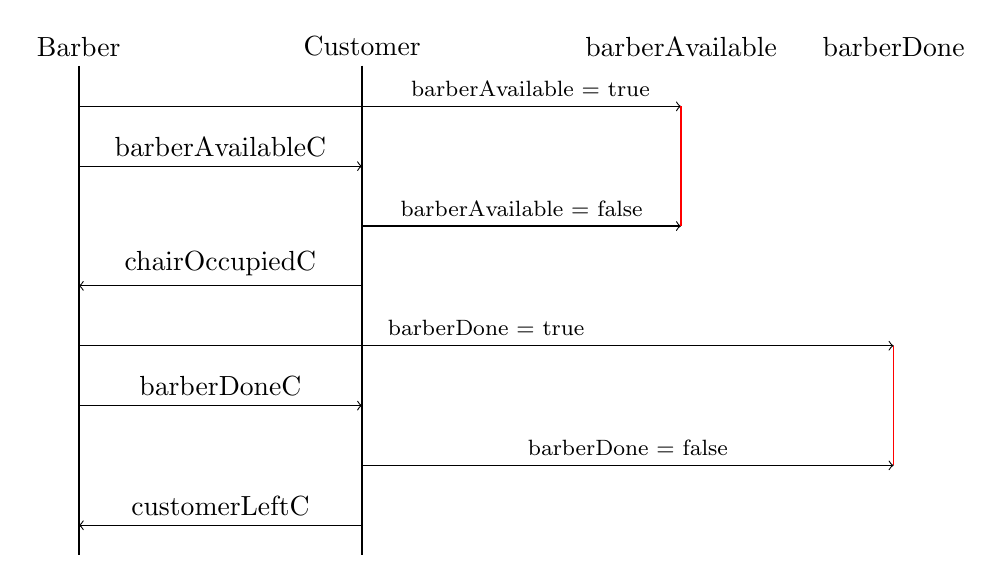
\begin{tikzpicture}[yscale = 0.76,xscale = 0.9]
\draw(0,0) node (b) {Barber};
\draw[black,thick] (b) -- ++ (0,-8.5);
\draw(\cx,0) node (c) {Customer};
\draw[black,thick] (c) -- ++ (0,-8.5);
\draw(\ba,0) node (ba) {\scalashape barberAvailable};
\draw(\bd,0) node (bd) {\scalashape barberDone};
%
\draw[->] (0,-1) -- 
  node[above,near end]{\footnotesize\scalashape barberAvailable = true}
  (\ba,-1);
\draw[->] (0,-2) -- node[above]{\scalashape barberAvailableC} (\cx,-2);
\draw[->] (\cx,-3) -- 
  node[above]{\footnotesize\scalashape barberAvailable = false}
  (\ba,-3);
\draw[red] (\ba,-1) -- (\ba,-3);
\draw[<-] (0,-4) -- node[above]{\scalashape chairOccupiedC} (\cx,-4);
%
\draw[->] (0,-5) -- node[above]{\footnotesize\scalashape barberDone = true}
   (\bd,-5);
\draw[->] (0,-6) -- node[above]{\scalashape barberDoneC} (\cx,-6);
\draw[->] (\cx,-7) -- node[above]{\footnotesize\scalashape barberDone = false}
   (\bd,-7);
\draw[red] (\bd,-5) -- (\bd,-7);
\draw[<-] (0,-8) -- node[above]{\scalashape customerLeftC} (\cx,-8);

\end{tikzpicture}
\end{slide}

%%%%%

\begin{slide}
\heading{The first two signals}

The barber signals that he is ready using |barberAvailableC|.  However, a
customer might not have arrived yet, so he also sets |barberAvailable|.  The
customer has to recheck |barberAvailable| when he awakes, in case another
customer has arrived and taken the slot. 

The barber then waits for a signal on |chairOccupiedC|.  There is only one
barber, and he must be waiting before the signal is sent, so nothing more is
needed. 
\end{slide}

%%%%%

\begin{slide}
\heading{The first two signals}

\begin{scala}
  /** Barber waits for next customer. */
  def getNextCustomer = lock.mutex{
    barberAvailable = true
    barberAvailableC.signal()                  // signal to a customer at (1)
    chairOccupiedC.await()                     // wait for signal (2)
  }

  /** Customer waits for barber to be available. */ 
  def getHaircut = lock.mutex{
    barberAvailableC.await(barberAvailable) // wait for barber (1)
    barberAvailable = false                   // clear for next round
    chairOccupiedC.signal()                   // signal to barber at (2)
  }
\end{scala}
\end{slide}

%%%%%

\begin{slide}
\heading{The third and fourth signals}

The barber signals he has finished on |barberDoneC|.  However, it's possible that
the customer isn't yet waiting, so he also sets |barberDone|.  No other
customer can be waiting on this signal, so nothing more is needed.

The barber then waits for a signal on |customerLeftC|.  Again he must be
waiting before the signal is sent, so nothing more is needed.
\begin{scala}
  def finishedCut = lock.mutex{
    barberDone = true; barberDoneC.signal()  // wake up customer at (3)
    customerLeftC.await()                        // wait for customer to leave (4)
  }

  def waitForHaircut = lock.mutex{
    if(!barberDone) barberDoneC.await()     // wait for barber to finish (3)
    assert(barberDone); barberDone = false  // clear for next round
    customerLeftC.signal()                     // signal to barber at (4)
  }
\end{scala}
\end{slide}




%%%%%
%%%%%%%%%%%%%%%%%%%%%%%%%%%%%%%%%%%%%%%%%%%%%%%%%%%%%%%
% \begin{slide}
% \heading{The status of the scenario}

% The scenario has four stages: the barber waiting for a customer; the customer
% sitting in the chair getting a haircut; the barber waiting for the customer to
% leave; the customer having left.   We therefore have a variable that records
% the current status:
% %
% \begin{scala}
% val barberAvailable = 0; 
% val chairOccupied = 1; 
% val doorOpen = 2; 
% val customerLeft = 3;
% var status = -1;
% \end{scala}
% \end{slide}

% %%%%%

% \begin{slide}
% \heading{The first two stages}

% The barber signals to a sleeping customer (if any), and waits until the chair
% is occupied.  The customer waits for the barber to be ready, occupies the
% chair, and signals to the barber.
% %
% \begin{scala}
% def GetNextCustomer = synchronized{
%   status = barberAvailable;
%   notify(); // wake up a sleeping customer
%   while(status!=chairOccupied) wait(); // wait for customer
% }

% def GetHaircut = synchronized{
%   while(status!=barberAvailable) wait(); // wait for barber
%   status = chairOccupied;
%   notifyAll(); // Signal to barber
% }
% \end{scala}
% \end{slide}

% %%%%%

% \begin{slide}
% \heading{The last two stages}

% The barber opens the door, signals to the customer, and waits for the customer
% to leave.  The customer waits for the barber to open the door, leaves, and
% signals to the barber.
% %
% \begin{scala}
% def FinishedCut = synchronized{
%   status = doorOpen;
%   notifyAll(); // signal to customer
%   while(status!=customerLeft) wait(); 
%     // wait for customer to leave
% }

% def WaitForHaircut = synchronized{
%   while(status!=doorOpen) wait(); // wait for barber to finish
%   status = customerLeft; 
%   notifyAll(); // Signal to barber
% }
% \end{scala}
% \end{slide}

% %%%%%

% \begin{selfnote}
% Note use of \SCALA{notifyAll()}

% Moral: identify the scenarios under which processes might be woken up; use
% state variables to ensure that processes wake up only under the appropriate
% circumstances, and only the appropriate number are woken up. 
% \end{selfnote}

%%%%%

\begin{slide}
\heading{Synchronisation problems}

Synchronisation problems like this can be difficult.  In order to come up with
a correct and understandable design, it is useful to use state variables that
indicate which processes are in different states, at least in \emph{quiescent
  states} when no processes
are running or runnable.

For example, the |barberAvailable| variable records (in quiescent states) that
the barber is waiting for a signal in |getNextCustomer|.  The customer that
will be served next clears this variable before signalling to the barber and
releasing the lock.

The |barberDone| variable records (in quiescent states) that the barber is
waiting for a signal in |finishedCut|.  The current customer clears this
variable before signalling to the barber and releasing the lock.
\end{slide}

%%%%%

% {\advance\slideheight by 3mm
% \begin{slide}
% \heading{Synchronisation problems}

% For example, with the sleeping barber, when no processes are running or
% runnable:
% %
% \begin{itemize}
% \item
% If \SCALA{barberAvailable = true} then the barber is waiting in
% \SCALA{GetNextCustomer} and no customers are in the module;

% \item
% If \SCALA{status == chairOccupied} then the barber is not in the module, one
% customer might be waiting in \SCALA{WaitForHaircut} (or has finished
% \SCALA{GetHairCut} and not yet started \SCALA{WaitForHairCut}), and other
% customers might be waiting in \SCALA{GetHairCut}.
% \end{itemize}
% %
% And
% %
% \begin{itemize}
% \item
% If \SCALA{status == doorOpen} then the barber is waiting in
% \SCALA{FinishedCut}, one customer is running or runnable in
% \SCALA{WaitForHairCut}, and other customers might be waiting in
% \SCALA{GetHairCut};

% \item
% If \SCALA{status == customerLeft} then the barber is running or runnable in
% \SCALA{FinishedCut}, or has exited \SCALA{FinishedCut}.
% \end{itemize}
% \end{slide}}

%%%%%

\begin{slide}
\heading{Synchronisation problems}

In other synchronisation problems, it can be useful to keep track of:
%
\begin{itemize}
\item 
How many processes are waiting in various waits;

\item
How many processes have completed operations (or maybe the difference between
the number of times two matching operations have been completed).
\end{itemize}

To track down bugs, it can be useful to:
\begin{itemize}
\item write lots of assertions;

\item use logging, particularly of the sending and receiving of
signals.
\end{itemize}
\end{slide}


%%%%%

\begin{slide}
\heading{Other languages}

Most other languages provide a mechanism similar to conditions.  For example
%
\begin{itemize}
\item Implementations of the Java interface
  |java.util.concurrent.locks.Condition|;

\item C++ |condition_variable|s.
\end{itemize}
%
Note that both of the above may suffer from spurious wake-ups.
\end{slide}

%%%%%

\begin{slide}
\heading{Summary}

\begin{itemize}
\item Conditions and targeted signals;

\item Examples;

\item Dealing with synchronisation problems.
\end{itemize}
\end{slide}
